\documentclass[12pt,addpoints]{repaso}
\grado{2}
\nivel{Primaria}
\cicloescolar{2024-2025}
\materia{Matemáticas}
\unidad{3}
\title{Practica la Unidad}
\aprendizajes{\scriptsize%
\item Expresa oralmente la sucesión numérica hasta cuatro cifras, en español y hasta donde sea posible, en su lengua materna, de manera ascendente y descendente a partir de un número natural dado.\\[-1.8em]
\item Representa, con apoyo de material concreto y modelos gráficos, fracciones: medios, cuartos, octavos, dieciseisavos, para expresar el resultado de mediciones y repartos en situaciones vinculadas a su contexto.\\[-1.8em]
\item Resuelve situaciones problemáticas vinculadas a su contexto que implican sumas, restas, multiplicación y división de números naturales de hasta tres cifras utilizando el algoritmo convencional y que impliquen, medición, estimación y comparación, de longitudes, masas y capacidades, con el uso del metro, kilogramo, litro y medios y cuartos de estas unidades; en el caso de la longitud, el decímetro y centímetro.\\[-1.8em]
   }
\author{Melchor Pinto, JC}
\begin{document}
\INFO%

% \begin{multicols}{2}
\tableofcontents
% \end{multicols}

\begin{questions}\large
	\addcontentsline{toc}{section}{Unidad 3}
	\section*{Unidad 3}

	\addcontentsline{toc}{subsection}{Tabla del 4}
	\subsection*{Tabla del 4}

	\questionboxed[6]{Contando de \textbf{4 en 4}, contesta las siguientes preguntas:

		\begin{multicols}{3}
			\begin{parts}\normalsize
				\part ¿qué número sigue del 12? \fillin[16][0.7cm]
				\part ¿qué número sigue del 28? \fillin[32][0.7cm]
				% \part ¿qué número sigue del 56? \fillin[60][0.7cm]
				\part ¿qué número sigue del 20? \fillin[24][0.7cm]
				% \part ¿qué número sigue del 18? \fillin[22][0.7cm]
				\part ¿qué número sigue del 36? \fillin[40][0.7cm]
				% \part ¿qué número sigue del 0?  \fillin[ 4][0.7cm]
				\part ¿qué número sigue del 8 ? \fillin[12][0.7cm]
				\part ¿qué número sigue del 21? \fillin[25][0.7cm]
				% \part ¿qué número sigue del 32? \fillin[36][0.7cm]
			\end{parts}
		\end{multicols}
	}

	\addcontentsline{toc}{subsection}{Tabla del 5}
	\subsection*{Tabla del 5}

	\questionboxed[6]{Contando de \textbf{5 en 5}, contesta las siguientes preguntas:

		\begin{multicols}{3}
			\begin{parts}\normalsize
				\part ¿qué número sigue del 12? \fillin[17][0.7cm]
				% \part ¿qué número sigue del 28? \fillin[33][0.7cm]
				\part ¿qué número sigue del 56? \fillin[61][0.7cm]
				\part ¿qué número sigue del 20? \fillin[25][0.7cm]
				% \part ¿qué número sigue del 18? \fillin[23][0.7cm]
				\part ¿qué número sigue del 36? \fillin[41][0.7cm]
				\part ¿qué número sigue del 0?  \fillin[ 5][0.7cm]
				% \part ¿qué número sigue del 7 ? \fillin[12][0.7cm]
				\part ¿qué número sigue del 21? \fillin[26][0.7cm]
				% \part ¿qué número sigue del 32? \fillin[37][0.7cm]
			\end{parts}
		\end{multicols}
	}

	\addcontentsline{toc}{subsection}{Tabla del 6}
	\subsection*{Tabla del 6}

	\questionboxed[6]{Contando de \textbf{6 en 6}, contesta las siguientes preguntas:

		\begin{multicols}{3}
			\begin{parts}\normalsize
				\part ¿qué número sigue del 12? \fillin[18][0.7cm]
				\part ¿qué número sigue del 28? \fillin[34][0.7cm]
				% \part ¿qué número sigue del 56? \fillin[62][0.7cm]
				\part ¿qué número sigue del 20? \fillin[26][0.7cm]
				\part ¿qué número sigue del 16? \fillin[22][0.7cm]
				% \part ¿qué número sigue del 34? \fillin[40][0.7cm]
				\part ¿qué número sigue del 0 ? \fillin[ 6][0.7cm]
				\part ¿qué número sigue del 6 ? \fillin[12][0.7cm]
				% \part ¿qué número sigue del 19? \fillin[25][0.7cm]
				% \part ¿qué número sigue del 30? \fillin[36][0.7cm]
			\end{parts}
		\end{multicols}
	}

	\questionboxed[12]{Reponde las siguientes tablas de multiplicar:

		\begin{multicols}{4}
			\begin{parts}
				\part $5 \times 9=$ \fillin[45][0.5cm]  
				\part $\fillin[6][0.5cm] \times 4= 24$  
				\part $5 \times 3=$ \fillin[15][0.5cm]  
				\part $5 \times \fillin[10][0.5cm]=50$  
				\part $3 \times 8=$ \fillin[24][0.5cm]  
				\part $4 \times \fillin[8][0.5cm]=32$  
				\part $6 \times 9=$ \fillin[54][0.5cm]  
				\part $4 \times \fillin[5][0.5cm]= 20$  
				\part $3 \times 6=$ \fillin[18][0.5cm]  
				\part $\fillin[2][0.5cm] \times 4= 8$  
				\part $2 \times 7=$ \fillin[14][0.5cm]  
				\part $4 \times \fillin[4][0.5cm]= 16$  
				\part $4 \times 7=$ \fillin[28][0.5cm]  
				\part $\fillin[3][0.5cm] \times 4= 12$  
				\part $3 \times 8=$ \fillin[24][0.5cm]  
				\part $4 \times \fillin[11][0.5cm]= 44$  
				\part $2 \times 9=$ \fillin[18][0.5cm]  
				\part $\fillin[9][0.5cm] \times 5= 45$  
				\part $4 \times 4=$ \fillin[16][0.5cm]  
				\part $4 \times \fillin[9][0.5cm]= 36$  
				\part $10 \times 3=$ \fillin[30][0.5cm]  
				\part $\fillin[7][0.5cm] \times 4= 28$  
				\part $7 \times 6=$ \fillin[42][0.5cm]  
				\part $\fillin[9][0.5cm] \times 3= 27$  
			\end{parts}
		\end{multicols}
	}

\newpage

	\addcontentsline{toc}{subsection}{Miselánea}
	\subsection*{Miselánea}

	\questionboxed[6]{Escribe sobre la línea el nombre que recibe cada figura geométrica de acuerdo con su número de lados:

		\begin{multicols}{3}
			\begin{parts}
				\part 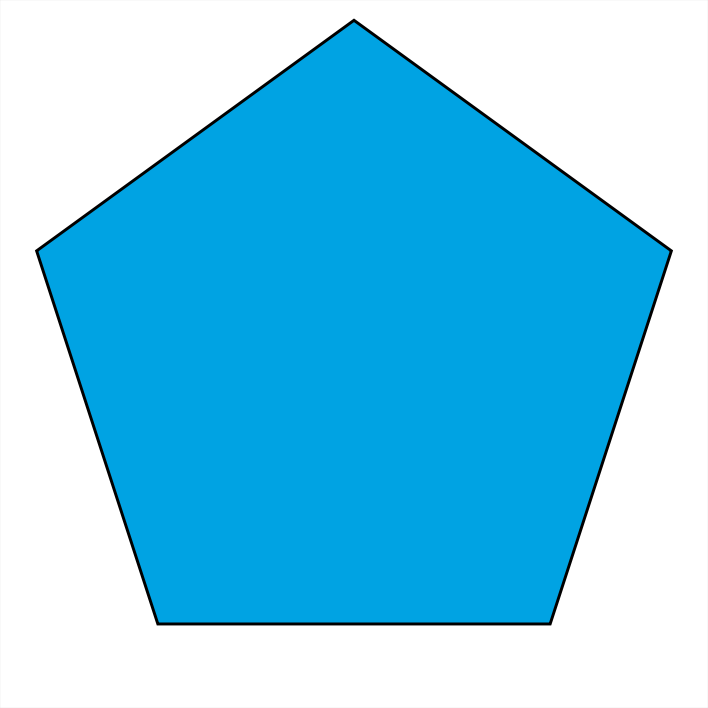
\includegraphics[width=75px]{../images/pentagono_azul.png}  \fillin[pentágono][0.75in]
				\part 
\includegraphics[width=75px]{../images/rombo_azul.png}   \fillin[rombo][0.75in]
				\part 
\includegraphics[width=75px]{../images/circulo_azul.png}   \fillin[círculo][0.75in]
				\part 
\includegraphics[width=75px]{../images/trapecio_azul.png}   \fillin[trapecio][0.75in]
				\part 
\includegraphics[width=75px]{../images/rectangulo_azul.png} \fillin[rectángulo][0.75in]
				\part 
\includegraphics[width=75px]{../images/cuadrado_azul.png}   \fillin[cuadrado][0.75in]
			\end{parts}
		\end{multicols}
	}

	\questionboxed[6]{Clasifica las siguientes fracciones en propias, impropias o mixtas:

		\begin{multicols}{4}
			\begin{parts}
				\part $\dfrac{5}{6}$   \fillin[Propia][1in]     \\[0.5em]
				\part $5\dfrac{5}{11}$ \fillin[Mixta][1in]      \\[0.5em]
				\part $\dfrac{13}{12}$   \fillin[Impropia][1in] \\[0.5em]
				\part $1\dfrac{2}{15}$  \fillin[Mixta][1in]     \\[0.5em]
				\part $\dfrac{42}{43}$   \fillin[Propia][1in]   \\[0.5em]
				\part $\dfrac{16}{9}$   \fillin[Impropia][1in]  \\[0.5em]
				\part $\dfrac{7}{3}$   \fillin[Impropia][1in]   \\[0.5em]
				\part $3\dfrac{2}{9}$  \fillin[Mixta][1in]      \\[0.5em]
				\part $\dfrac{3}{2}$   \fillin[Impropia][1in]   \\[0.5em]
				\part $1\dfrac{2}{3}$  \fillin[Mixta][1in]      \\[0.5em]
				\part $\dfrac{7}{8}$   \fillin[Propia][1in]     \\[0.5em]
				\part $\dfrac{6}{5}$   \fillin[Impropia][1in]   \\[0.5em]
			\end{parts}
		\end{multicols}
	}

	\questionboxed[6]{Escribe sobre la línea la fracción que representa cada imagen:

		\begin{multicols}{5}
			\begin{parts}
				\part 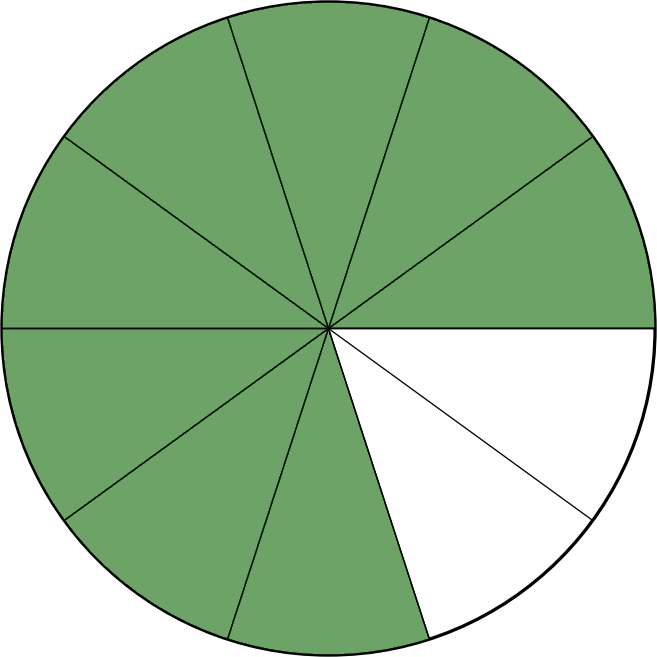
\includegraphics[width=0.7\linewidth]{../images/imagen_frac_2prim_8|10.png}  \fillin[$\sfrac{8}{10}$][0.5cm] \\[-0.5em]
				\part 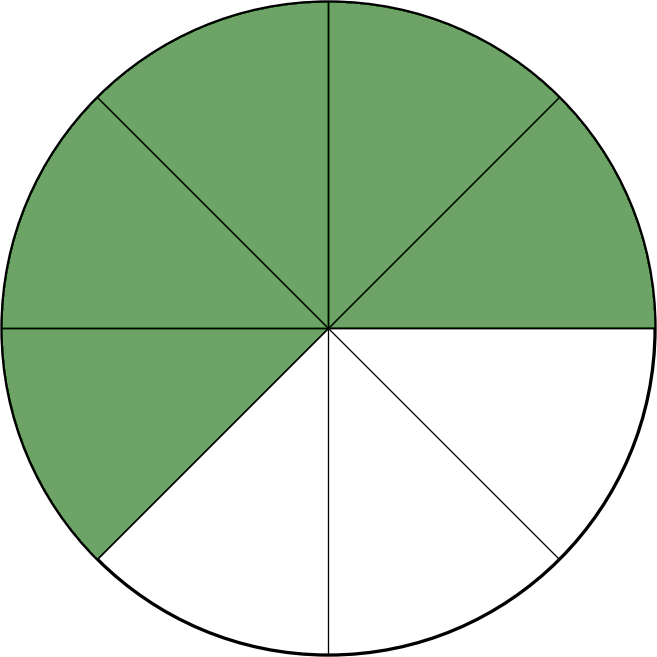
\includegraphics[width=0.7\linewidth]{../images/imagen_frac_2prim_5|8.png}   \fillin[$\sfrac{5}{8}$ ][0.5cm] \\[-0.5em]
				\part 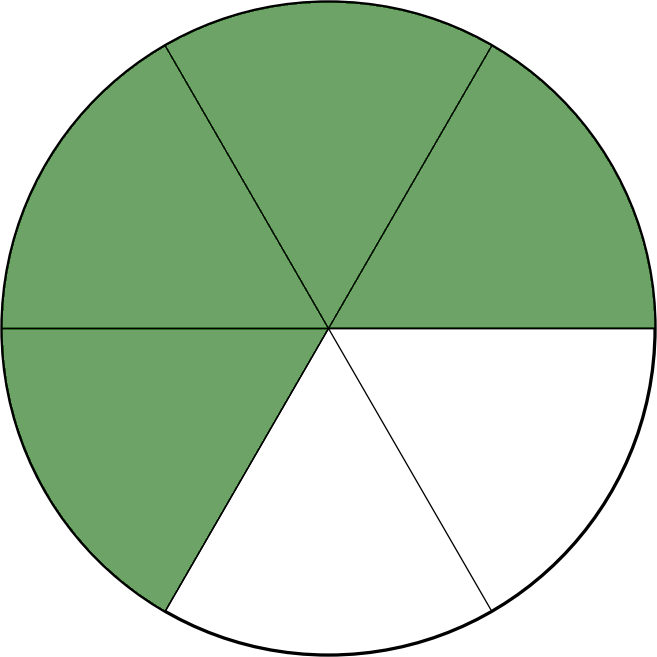
\includegraphics[width=0.7\linewidth]{../images/imagen_frac_2prim_4|6.png}   \fillin[$\sfrac{4}{6}$ ][0.5cm] \\[-0.5em]
				\part 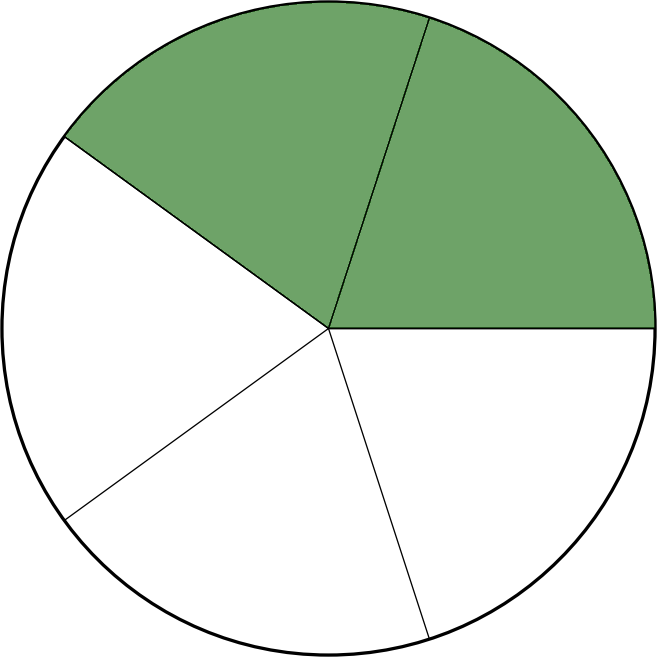
\includegraphics[width=0.7\linewidth]{../images/imagen_frac_2prim_2|5.png}   \fillin[$\sfrac{2}{5}$ ][0.5cm] \\[-0.5em]
				\part 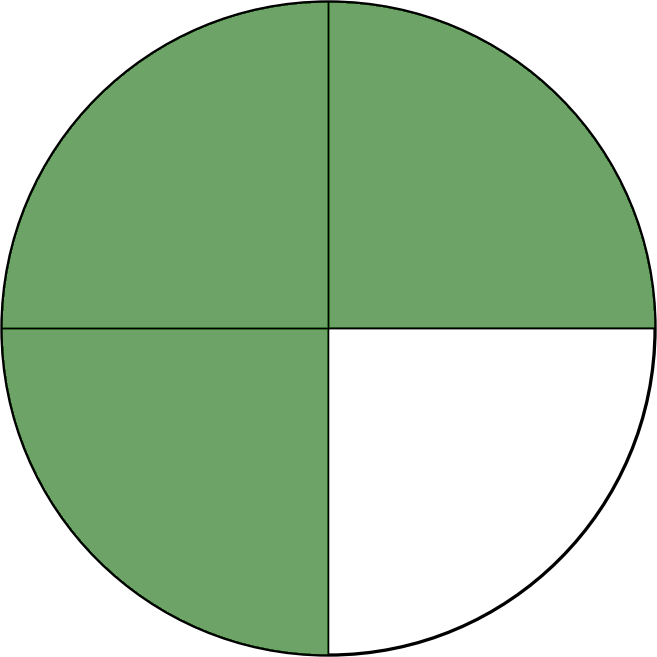
\includegraphics[width=0.7\linewidth]{../images/imagen_frac_2prim_3|4.png}   \fillin[$\sfrac{3}{4}$ ][0.5cm] \\[-0.5em]
				\part 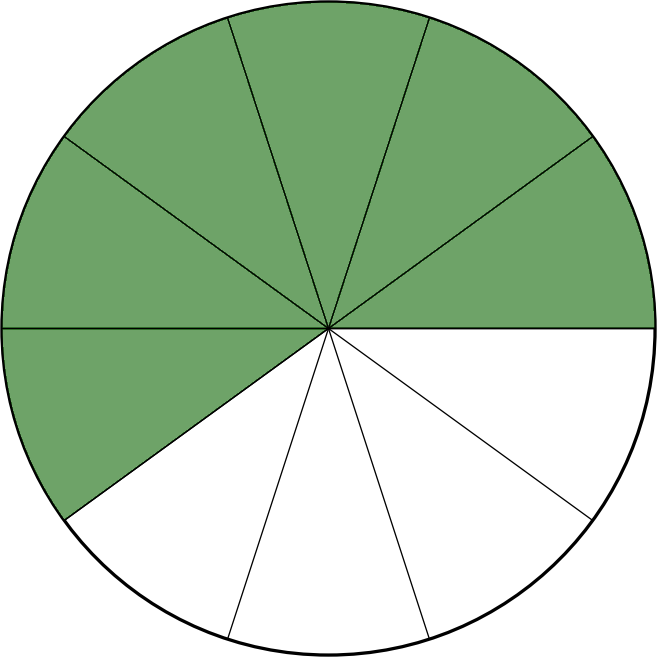
\includegraphics[width=0.7\linewidth]{../images/imagen_frac_2prim_6|10.png}  \fillin[$\sfrac{6}{10}$][0.5cm] \\[-0.5em]
				\part 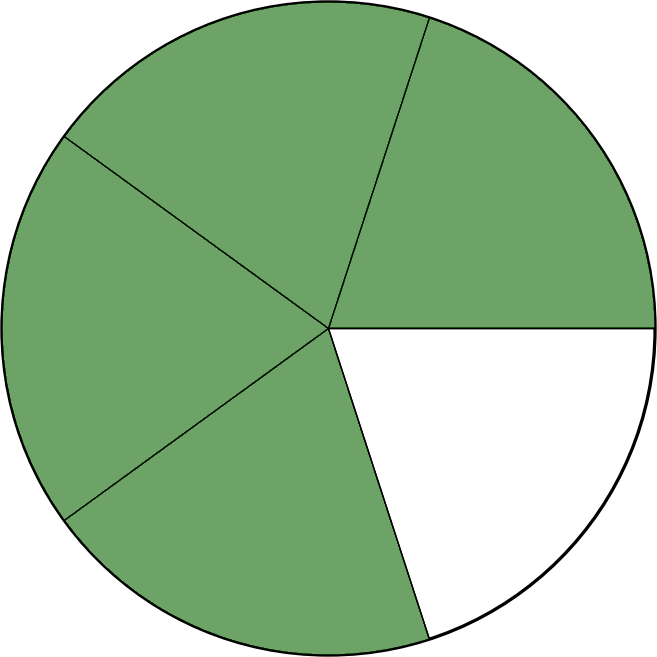
\includegraphics[width=0.7\linewidth]{../images/imagen_frac_2prim_4|5.png}   \fillin[$\sfrac{4}{5}$ ][0.5cm] \\[-0.5em]
				\part 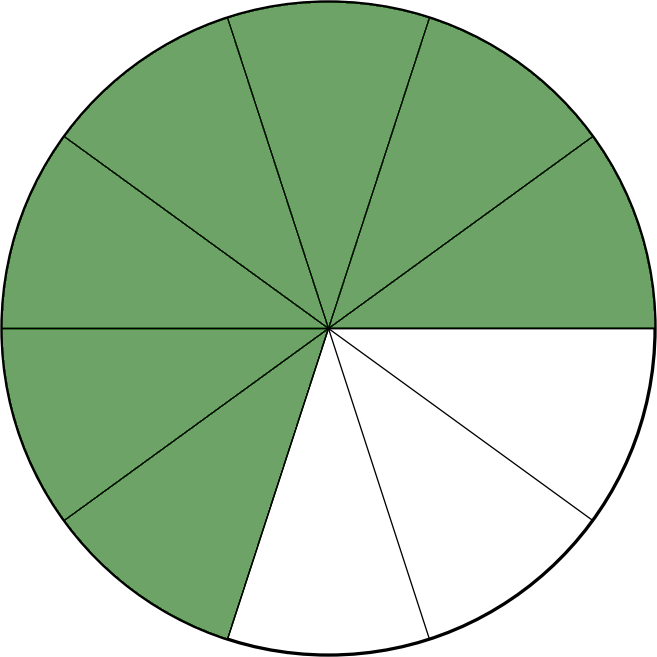
\includegraphics[width=0.7\linewidth]{../images/imagen_frac_2prim_7|10.png}  \fillin[$\sfrac{7}{10}$][0.5cm] \\[-0.5em]
				\part 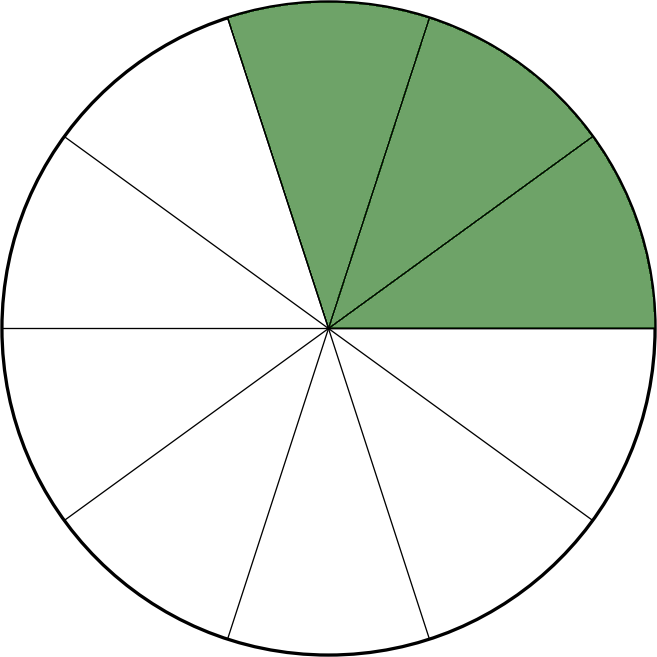
\includegraphics[width=0.7\linewidth]{../images/imagen_frac_2prim_3|10.png}  \fillin[$\sfrac{3}{10}$][0.5cm] \\[-0.5em]
				\part 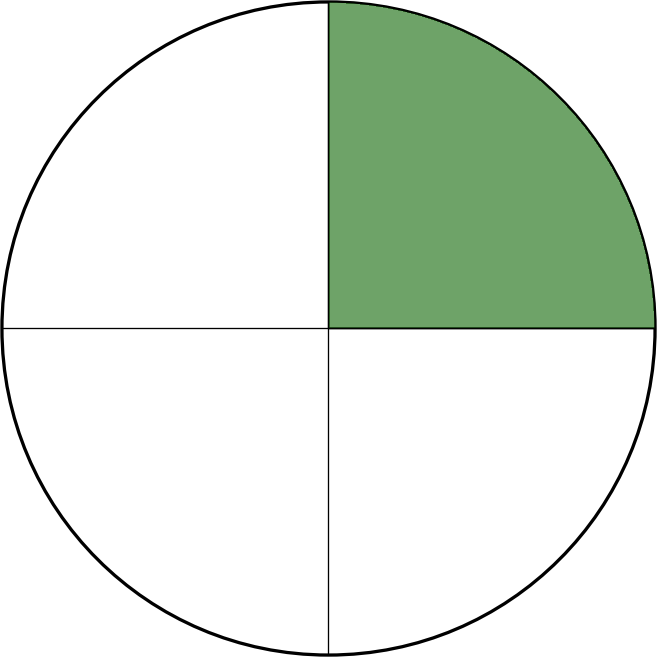
\includegraphics[width=0.7\linewidth]{../images/imagen_frac_2prim_1|4.png}   \fillin[$\sfrac{1}{4}$ ][0.5cm] \\[-0.5em]
			\end{parts}
		\end{multicols}
	}

\end{questions}
\end{document}